\documentclass[journal,12pt,twocolumn]{IEEEtran}
%
\usepackage{setspace}
\usepackage{gensymb}
\usepackage{caption}
%\doublespacing
\singlespacing
%\usepackage{graphicx}
%\usepackage{amssymb}
%\usepackage{relsize}
\usepackage[cmex10]{amsmath}
%\usepackage{amsthm}
%\interdisplaylinepenalty=2500
%\savesymbol{iint}
%\usepackage{txfonts}
%\restoresymbol{TXF}{iint}
%\usepackage{wasysym}
\usepackage{amsthm}
%\usepackage{iithtlc}
\usepackage{mathrsfs}
\usepackage{txfonts}
\usepackage{stfloats}
\usepackage{bm}
\usepackage{cite}
\usepackage{cases}
\usepackage{subfig}
\usepackage{xtab}
\usepackage{multirow}
%\usepackage{algorithm}
%\usepackage{algpseudocode}
\usepackage{booktabs}
\usepackage{enumitem}
\usepackage{mathtools}
\usepackage{tikz}
\usepackage{pgfplots}
\usepackage{circuitikz}
\usepackage{verbatim}
\usepackage{tfrupee}
\usepackage[breaklinks=true]{hyperref}
%\usepackage{stmaryrd}
\usepackage{tkz-euclide} % loads  TikZ and tkz-base
%\usetkzobj{all}
\usetikzlibrary{fit}
\usetikzlibrary{calc,math}
%\pgfdeclarelayer{background}
%\pgfsetlayers{background}
\usepackage{listings}
    \usepackage{color}                                            %%
    \usepackage{array}                                            %%
    \usepackage{longtable}                                        %%
    \usepackage{calc}                                             %%
    \usepackage{multirow}                                         %%
    \usepackage{hhline}                                           %%
    \usepackage{ifthen}                                           %%
  %optionally (for landscape tables embedded in another document): %%
    \usepackage{lscape}     
\usepackage{multicol}
\usepackage{chngcntr}
%\usepackage{enumerate}

%\usepackage{wasysym}
%\newcounter{MYtempeqncnt}
\DeclareMathOperator*{\Res}{Res}
%\renewcommand{\baselinestretch}{2}
\renewcommand\thesection{\arabic{section}}
\renewcommand\thesubsection{\thesection.\arabic{subsection}}
\renewcommand\thesubsubsection{\thesubsection.\arabic{subsubsection}}

\renewcommand\thesectiondis{\arabic{section}}
\renewcommand\thesubsectiondis{\thesectiondis.\arabic{subsection}}
\renewcommand\thesubsubsectiondis{\thesubsectiondis.\arabic{subsubsection}}

% correct bad hyphenation here
\hyphenation{op-tical net-works semi-conduc-tor}
\def\inputGnumericTable{}                                 %%

\lstset{
%language=C,
frame=single, 
breaklines=true,
columns=fullflexible
}
%\lstset{
%language=tex,
%frame=single, 
%breaklines=true
%}

\begin{document}
%


\newtheorem{theorem}{Theorem}[section]
\newtheorem{problem}{Problem}
\newtheorem{proposition}{Proposition}[section]
\newtheorem{lemma}{Lemma}[section]
\newtheorem{corollary}[theorem]{Corollary}
\newtheorem{example}{Example}[section]
\newtheorem{definition}[problem]{Definition}
%\newtheorem{thm}{Theorem}[section] 
%\newtheorem{defn}[thm]{Definition}
%\newtheorem{algorithm}{Algorithm}[section]
%\newtheorem{cor}{Corollary}
\newcommand{\BEQA}{\begin{eqnarray}}
\newcommand{\EEQA}{\end{eqnarray}}
\newcommand{\define}{\stackrel{\triangle}{=}}
\newcommand{\RomanNumeralCaps}[1]
    {\MakeUppercase{\romannumeral #1}}
\bibliographystyle{IEEEtran}
%\bibliographystyle{ieeetr}
\providecommand{\mbf}{\mathbf}
\providecommand{\pr}[1]{\ensuremath{\Pr\left(#1\right)}}
\providecommand{\qfunc}[1]{\ensuremath{Q\left(#1\right)}}
\providecommand{\sbrak}[1]{\ensuremath{{}\left[#1\right]}}
\providecommand{\lsbrak}[1]{\ensuremath{{}\left[#1\right.}}
\providecommand{\rsbrak}[1]{\ensuremath{{}\left.#1\right]}}
\providecommand{\brak}[1]{\ensuremath{\left(#1\right)}}
\providecommand{\lbrak}[1]{\ensuremath{\left(#1\right.}}
\providecommand{\rbrak}[1]{\ensuremath{\left.#1\right)}}
\providecommand{\cbrak}[1]{\ensuremath{\left\{#1\right\}}}
\providecommand{\lcbrak}[1]{\ensuremath{\left\{#1\right.}}
\providecommand{\rcbrak}[1]{\ensuremath{\left.#1\right\}}}
\theoremstyle{remark}
\newtheorem{rem}{Remark}
\newcommand{\sgn}{\mathop{\mathrm{sgn}}}
\providecommand{\res}[1]{\Res\displaylimits_{#1}} 
%\providecommand{\norm}[1]{\lVert#1\rVert}
\providecommand{\mtx}[1]{\mathbf{#1}}
\providecommand{\fourier}{\overset{\mathcal{F}}{ \rightleftharpoons}}
%\providecommand{\hilbert}{\overset{\mathcal{H}}{ \rightleftharpoons}}
\providecommand{\system}{\overset{\mathcal{H}}{ \longleftrightarrow}}
	%\newcommand{\solution}[2]{\textbf{Solution:}{#1}}
\newcommand{\solution}{\noindent \textbf{Solution: }}
\newcommand{\cosec}{\,\text{cosec}\,}
\providecommand{\dec}[2]{\ensuremath{\overset{#1}{\underset{#2}{\gtrless}}}}
\newcommand{\myvec}[1]{\ensuremath{\begin{pmatrix}#1\end{pmatrix}}}
\newcommand{\mydet}[1]{\ensuremath{\begin{vmatrix}#1\end{vmatrix}}}
\newcommand*{\permcomb}[4][0mu]{{{}^{#3}\mkern#1#2_{#4}}}
\newcommand*{\perm}[1][-3mu]{\permcomb[#1]{P}}
\newcommand*{\comb}[1][-1mu]{\permcomb[#1]{C}}
%\newcommand*{\perm}[2]{{}^{#1}\!P_{#2}}%
%\newcommand*{\comb}[2]{{}^{#1}C_{#2}}%
%\numberwithin{equation}{section}
\numberwithin{equation}{subsection}
%\numberwithin{problem}{section}
%\numberwithin{definition}{section}
\makeatletter
\@addtoreset{figure}{problem}
\makeatother
\let\StandardTheFigure\thefigure
\let\vec\mathbf
%\renewcommand{\thefigure}{\theproblem.\arabic{figure}}
\renewcommand{\thefigure}{\theproblem}
%\setlist[enumerate,1]{before=\renewcommand\theequation{\theenumi.\arabic{equation}}
%\counterwithin{equation}{enumi}
%\renewcommand{\theequation}{\arabic{subsection}.\arabic{equation}}
\def\putbox#1#2#3{\makebox[0in][l]{\makebox[#1][l]{}\raisebox{\baselineskip}[0in][0in]{\raisebox{#2}[0in][0in]{#3}}}}
     \def\rightbox#1{\makebox[0in][r]{#1}}
     \def\centbox#1{\makebox[0in]{#1}}
     \def\topbox#1{\raisebox{-\baselineskip}[0in][0in]{#1}}
     \def\midbox#1{\raisebox{-0.5\baselineskip}[0in][0in]{#1}}
\vspace{3cm}
\title{Assignment 2}
\author{Namita Kumari - CS20BTECH11034}
\maketitle
\newpage
\bigskip
Download all python codes from 
\begin{lstlisting}
https://github.com/ImNamitaKumari/Probability-and-Random-Variables/blob/main/Assignment2/codes/Assignment2.py
\end{lstlisting}
%
and latex-tikz codes from 
%
\begin{lstlisting}
https://github.com/ImNamitaKumari/Probability-and-Random-Variables/blob/main/Assignment2/Assignment2.tex
\end{lstlisting}
\section{Problem}
62) Suppose the random variable $U$ has uniform distribution on [0,1] and $X=-2\log{U}$. The density of $X$ is:
\begin{enumerate}
\item $f(x)=$
$\begin{cases}
e^{-x} & x>0\\
0 & \mathrm{otherwise}
\end{cases}$

\item $f(x)=$
$\begin{cases}
2e^{-2x} & x>0\\
0 & \mathrm{otherwise}
\end{cases}$

\item $f(x)=$
$\begin{cases}
\frac{1}{2}e^{-\frac{x}{2}} & x>0\\
0 & \mathrm{otherwise}
\end{cases}$

\item $f(x)=$
$\begin{cases}
\frac{1}{2} & x\in [0,2]\\
0 & \mathrm{otherwise}
\end{cases}$
\end{enumerate}
\section{solution}
$U$ has a uniform distribution in [0,1].
\begin{align}
    \implies \mathrm{PDF(U)}=f_U(x)=k, k\in\textbf{N}, x\in[0,1]
\end{align}
Now,
\begin{align}
    \int_{0}^1 f_U(x)\,dx=1\\
    \implies f_U(x)=1, \forall x\in[0,1]\label{2.0.6}
\end{align}
\begin{align}
    X=-2\log{U},U\in[0,1]\\
    \implies X\in[0,\infty)\label{eq: 0}
\end{align}
CDF of X will be given by,
\begin{align}
F_{X}(x) = \pr{X\leq x}  
\end{align}
Here, from \eqref{eq: 0},
\begin{align}
x\in[0,\infty)
    \implies e^{-\frac{x}{2}}\in [0,1]\label{eq: 2.0.8}
\end{align}
\begin{multline}
    \implies F_X(x)  =\pr{-2\log U\leq x} 
    =\pr{U\geq e^{-\frac{x}{2}}}\\
    =1-\pr{U\leq e^{-\frac{x}{2}}}\\
    =1-F_{U}(e^{-\frac{x}{2}})\label{eq: 2.0.9}
    \end{multline}
We know that,
\begin{align}
    \mathrm{PDF}=f(x)=\frac{d[\mathrm{F}(x)]}{dx}
\end{align}
Differentiating both sides of \eqref{eq: 2.0.9}, we get
\begin{align}
    \frac{d[\mathrm{F}_X(x)]}{dx}=-\frac{d[\mathrm{F}_U(e^{-\frac{x}{2}})]}{dx}\label{eq: 2.0.3}\\
    \implies f_{X}(x)=-f_{U}(e^{-\frac{x}{2}})\brak{\frac{de^{-\frac{x}{2}}}{dx}}
    \end{align}
  From \eqref{2.0.6},
  \begin{align}
      f_X(x)=-1\times \brak{e^{-\frac{x}{2}}}\brak{-\frac{1}{2}}=\frac{1}{2}e^{-\frac{x}{2}},x\in[0,\infty)
  \end{align}
  Hence,
  \begin{align}
  f_X(x)=
\begin{cases}
\frac{1}{2}e^{-\frac{x}{2}} & x\geq0\\
0 & \mathrm{otherwise}
\end{cases}
\end{align}
\begin{figure}[h]
\begin{center}
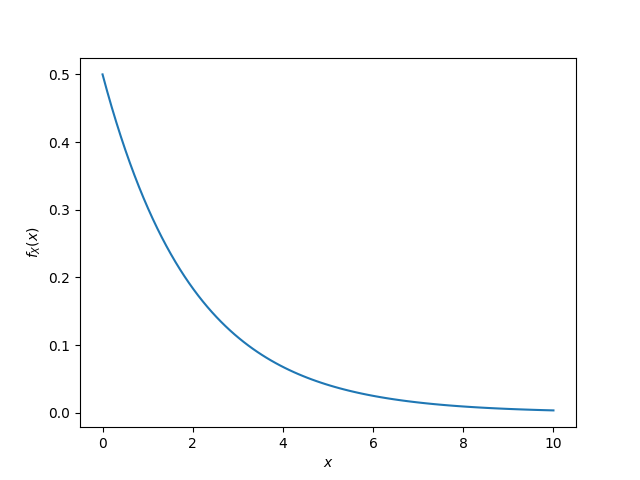
\includegraphics[scale=0.45]{Figure_1.png}
\end{center}
\caption{PDF of random variable X}\label{fig1}
\end{figure}
\end{document}
